\subsection{Cavity Line Model}
\indent The cavity model has more accurate formulation for the input impedance, resonance with a little
        increase of mathematical complexity.\cite{CaM:81}
\begin{figure}[ht]
  \label{cavitymodel}
  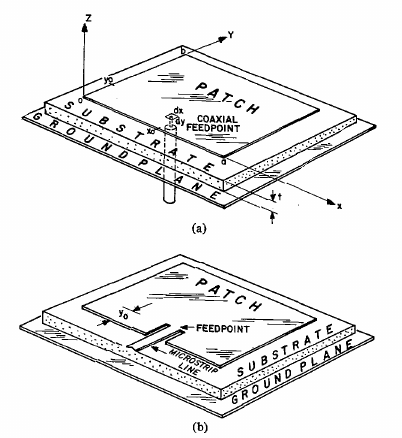
\includegraphics{cavitymodel.png}
  \centering
  \caption{(a) Microstrip patch with inset coaxial feed
           (b) Microstrip patch with inset transmission-line feed
          }
\end{figure}

  \subsubsection{General form of electric field}
    \indent Considering a rectangular patch with width $a$ and length $b$ over a ground plane with $t$ substrate
            thickness and a dielectric constant $\epsilon_r$. With the relatively short thickness of the substrate,
            the electric field will be in z-direction with $TM_{mn}$ interior modes so that\cite{CaM:81}
    \begin{equation}
      \label{GeneralE}
      E_z = \sum_m\sum_n A_{mn}e_{mn}(x,y)
    \end{equation}
    \indent where $A_{mn}$ are the mode amplitude coefficients and $e_{mn}$ are z direction electric mode vectors.
    \indent However, the mode that is used in the antenna is just only $TM_{10}$ so the equation can easily write as
    \begin{equation}
       E_z = A_{10}e_{10}(x,y)
    \end{equation}

  \subsubsection{Nonradiating cavity with perfect open-circuit wall equation of electric field}
    \indent With a calculation from boundary condition, it could be found that
      \begin{equation}
        \label{OpenE}
        e_{mn}(x,y) = \frac{\chi_{mn}}{\sqrt{\epsilon abt}}\cos{k_nx}\cos{k_my}
      \end{equation}
    \indent with
      \begin{equation}
        \chi_{mn}=
        \begin{cases}
          1       , & m = 0\quad     \text{and}\quad  n = 0 \\
          \sqrt{2}, & m = 0\quad     \text{ or }\quad  n = 0 \\
          2       , & m \neq 0\quad  \text{and}\quad  n \neq 0
        \end{cases}
      \end{equation}

  \subsubsection{Wavenumber}
    \indent The homogenous wave function and the eigenvalues must be complied with the seperation equation
    \begin{equation}
      \label{kmn}
      k_{mn}^2 = \omega_{mn}^2\mu\epsilon = k_n^2 + k_m^2\\
    \end{equation}
    \indent in the case of nonradiating cavity
    \begin{equation}
      k_{n} = \frac{n\pi}{a}\\
      k_{m} = \frac{m\pi}{b}
    \end{equation}

  \subsubsection{Nonradiating cavity with perfect open-circuit wall equation of magnetic field}
    \indent From Maxwell-Faraday equation
    \begin{equation}
      \nabla \times \vv{E} = - \frac {\partial{\vv B}} {\partial t}
    \end{equation}
    \indent or in phasor form,
    \begin{equation}
      \nabla \times \vv{E} = -j\omega{\vv B}
    \end{equation}
    \indent after substitute the electric field equation, the magnetic field will be
    \begin{equation}
       \vv{h}_{mn} = \frac{1}{j\omega\mu}\frac{\chi_{mn}}{\sqrt{\epsilon abt}}(\vv{x}k_m\cos{k_nx}\sin{k_my} - \vv{y}k_n\sin{k_n}{x}\cos{k_m}{y})
    \end{equation}
    \indent For nonradiating case, the boundary condition $\vv{n} \times \vv{h}_{mn} = 0$ is satisfied on every walls.
            But, in radiating case, $\vv{h}_{mn}$ will not have a zero tangential on the cavity sidewall anymore.
            However, those pertubation from radiating effect cause just a little error on $e_{mn}$\cite{CaM:81}
  
  \subsubsection{Mode Coefficient}
    \indent From z-direction current, with the current probe $I_{0}$ at the location $(x_0,y_0)$ as in the
            figures illustrates in \ref{cavitymodel}. The coefficients from each mode can be obtained from
    \begin{equation}
      A_{mn} = \frac{j\sqrt{\mu\epsilon}k}{k^2-k_{mn}^2} \int\int\int\vv{J} \cdot \vv{e}_{mn} dv
    \end{equation}
    \begin{equation}
      \label{ModeCoeff}
      A_{mn} = jI_0 \sqrt{\frac{\mu t}{ab}} \frac{k\chi_{mn}}{k^2-k_{mn}^2} G_{mn} \cos{k_my_0}\cos{k_nx_0}
    \end{equation}
    \indent where
    \begin{equation}
      G_{mn} = \frac{\sin(n\pi d_x/2a)}{n\pi d_x/2a}\frac{\sin(m\pi d_y/2b)}{m\pi d_y/2b}
    \end{equation}
    \indent and
    \begin{equation}
      k_{mn} = \widetilde{\omega}\sqrt{\mu\epsilon}
    \end{equation}
    \indent $\widetilde{\omega}$ is the complex resonance frequency of the $mn$th mode which could found by \ref{kmn}

    \subsubsection{Complete Electric Field form}
      \indent After combining \ref{GeneralE} \ref{OpenE} \ref{ModeCoeff} altogether, the complete electric field form will be
      \begin{equation}
        E_z(x,y) = jI_0Z_0k \sum_{m=0}^{\infty} \sum_{n=0}^{\infty} \frac{\psi_{mn}(x,y)\psi_{mn}(x_0,y_0)}{k^2-k_{mn}^2}G_{mn}
      \end{equation}
    
      \indent where $Z_0 = \sqrt{\mu}{\epsilon}$, $k = \omega\sqrt{\mu\epsilon}$, $k_{mn}^2 = k_{m}^2 + k_{n}^2$ and
      \begin{eqnarray}
        \psi_{mn} &=& \frac{\chi_{mn}}{\sqrt{ab}}\cos{k_nx}\cos{k_my} \nonumber \\
                  &=& \frac{\chi_{mn}}{\sqrt{ab}}\cos{\frac{n\pi x}{a}}\cos{\frac{m\pi y}{b}}
      \end{eqnarray}
    \subsubsection{Voltage at the feeding point}
      \indent From $E = - \nabla V$, or rewrite as $V = -Ed$, the voltage at the feeding point will be
      \begin{eqnarray}
          V_{in} &=& -tE_z(x_0,y_0) \nonumber \\
                &=& -jI_0Z_0k \sum_{m=0}^{\infty} \sum_{n=0}^{\infty} \frac{\psi_{mn}^2(x_0,y_0)}{k^2-k_{mn}^2} G_{mn}
      \end{eqnarray}
    \subsubsection{Input Resistance}
      \indent From Ohm's law, $V = IR$, the input impedance is
      \begin{equation}
        Z_{in} = \frac{V_{in}}{I_0} = -jZ_0k \sum_{m=0}^{\infty} \sum_{n=0}^{\infty} \frac{\psi_{mn}^2(x_0,y_0)}{k^2-k_{mn}^2} G_{mn}
      \end{equation}
    
    \subsubsection{Summary}
      \indent From this model, cavity model, it's found that this has more accurary than the transmission line
              because it has less approximation and it has more calculation complexity
    